\section{Processi di supporto}

\subsection{Documentazione}

\subsubsection{Scopo}
Lo scopo di questa sezione è definire gli standard neccessari per la stesura di tutti i documenti del progetto.

\subsubsection{Ciclo di vita del documento}
Tutti i documenti prodotti dal team seguono la seguente ciclo di vita:
\begin{itemize}
    \item \textbf{Stesura}: il documento viene scritto utilizzando il metodo AGILE, adottando gli sprint di durata una settimana; 
    \item \textbf{Revisione}:a fine di ogni sprint i documenti vengono revisionati da una persona diversa dal redattore. Solo dopo la revisione
				le modifiche e i nuovi contenuti scritti possono essere integrati nel documento;
    \item \textbf{Verifica}:avviene in un periodo specificato nel piano di progetto, tale attività viene svolto da almeno una persona. Il documento
				è considerato verificato quando i Verificatori dichiarano che le modifiche neccessarie sono portate a termine;
    \item \textbf{Approvazione}:il Responsabile di Progetto dichiara che il documento è completo in ogni sua
					parte e pronto per essere rilasciato, marcandolo come approvato;
\end{itemize}
\begin{figure}[H]
    \centering
    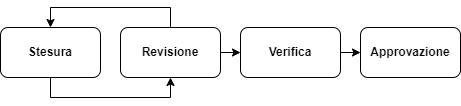
\includegraphics[scale=0.8]{img/ciclo_di_vita.png}
    \caption{Ciclo di vita dei documenti}
\end{figure}

\subsubsection{Struttura dei documenti}
Tutti i documenti ufficiali seguono una struttura ben definita cosi da mantenere l'omogeneità. Più precisamente ogni documento è formato da:
\begin{itemize}
    \item \textbf{Fontespizio};
    \item \textbf{Registro delle modifiche};
    \item \textbf{Indice};
    \item \textbf{Contenuto principale}.
\end{itemize}

\subsubsubsection{Fontespizio}
Rappresenta la pagina iniziale del documento ed è strutturato come segue:
\begin{itemize}
    \item \textbf{Logo dell'università}: logo dell'\textit{Università di Padova} posizionato in centro alto della pagina, seguito dalla nomenclatura "Università degli  Studi di Padova";
    \item \textbf{Logo del gruppo}: logo del gruppo, posizionato in centro, subito dopo la nomeclatura dell'università;
    \item \textbf{Nome del gruppo e del progetto}: il nome del gruppo e del capitolato scelto, seguito da un recapito email;
    \item \textbf{Nome del documento}: è il titolo del documento, definito in grassetto e posizionato al centro della pagina;
    \item \textbf{Tabella di descrizione}: è la tabella contenente le informazioni generali del documento.
\end{itemize}

\subsubsubsection{Registro delle modifiche}
I documenti che sono soggetti a modifiche periodiche sono dotati di un registro che ne memorizza lo storico. Il registro è fomato cosi:
\begin{itemize}
    \item \textbf{Versione}: indica la versione del documento dopo la modifica;
    \item \textbf{Descrizione}: descrive brevemente la modifica apportata;
    \item \textbf{Data}: indica la data in cui è stata modificata il documento.
\end{itemize}

\subsubsubsection{Indice}
Per agevolare la lettura, tutti i documenti sono dotati di un indice. Le sezioni sono rappresentati da un numero seguiti dal titolo della sezione, ogni sottosezione deve riportare il numero della sezione madre e poi il numero proprio. I numeri devono partire dall'1.

\subsubsubsection{Contenuto principale}
La pagina del contenuto è costituita da:
\begin{itemize}
    \item \textbf{Intestazione}: in alto a sinistra deve esserci il nome del gruppo \textit{Catch em All}, in altro a destra si trova il numero e nome della sezione in cui si trova;
    \item \textbf{Pie di pagina}: in basso sinistra si trova il nome del documento e la sua versione attuale, in basso a destra viene indicato il numero della pagina in cui si trova e il numero di pagine complessive del documento.
\end{itemize}

\subsubsection{Classificazione dei documenti}
Tutti i documenti prodotti sono divisi in uso interno e uso esterno:
\begin{itemize}
    \item \textbf{Uso interno}: sono documenti finalizzati a un uso interno al gruppo, tra cui \textit{Norme di progetto} e \textit{Verbali interni};
    \item \textbf{Uso esterno}: sono documenti di interesse a tutti gli stakeholder, tra cui \textit{Analisi dei requisiti}, \textit{Verbali esterni}, \textit{Piano di progetto}, (da completare).
\end{itemize}

\subsubsection{Norme tipografiche}

\subsubsubsection{Nome del file}
Di seguito viene descritto il formato dei nomi dei documenti:
\begin{itemize}
\item Iniziano tutti con la lettera minuscola;
\item Se il nome comprende più parole allora ognuna di esse è separata dal simbolo '\_';
\item Deve essere seguito da un indicazione della propria versione.
\end {itemize}
La sigla della versione deve essere così strutturata:
\begin{center}
    \large{\textbf{v.X.Y.Z}}
\end{center}
\begin{itemize}
\item \textbf{X} indicato da un numero che parte da 0, corrisponde al numero di approvazioni del documento da parte del responsabile;
\item \textbf{Y} indicato da un numero che parte da 0, corrisponde al numero di verifiche del documento da parte del verificatore, viene portato a 0 ad ogni incremento di \textbf{X};
\item \textbf{Z} indicato da un numero che parte da 0, corrisponde al numero di modifiche del documento da parte del redattore, viene portato a 0 ad ogni incremento di \textbf{X} e \textbf{Y}.
\end {itemize}
Esempi corretti: introduzione\textunderscore v0.0.1; norme\textunderscore di\textunderscore progetto\textunderscore v.0.0.1 .\\
Esempi non corretti: Norme\textunderscore di\textunderscore Progetto; NormeDiProgetto.

I verbali non seguono questa norma e hanno una nomenclatura diversa, poichè non subiscono variazioni dopo la prima redazione e hanno il seguente formato: (DA DEFINIRE)

\subsubsubsection{Stile di testo}
Di seguito vengono riportati i vari stili del testo e i loro usi:
\begin {itemize}
\item \textbf{Grassetto}: viene utilizzato per i termini negli elenchi puntati e per i titoli delle sezioni;
\item \textbf{Corsivo}: viene utilizzato per il nome del gruppo, l'email del gruppo e il nome del progetto;
\item \textbf{Link}: i link sono collegamenti esterni del documento.
\end {itemize}

\subsubsubsection{Glossario}
Le norme relative al \textit{Glossario} sono:
\begin{itemize}
    \item Ogni parola presente nel \textit{glossario} viene contrassegnata con una 'G' a pedice;
    \item Se un termine compare nella sua stessa definizione all'interno del \textit{glossario} esso viene contrassegnato.
\end{itemize}

\subsubsubsection{Elenchi puntati e numerati}
Di seguito vengono descritti come vengono utilizzati gli elenchi puntati e numerati:
\begin {itemize}
\item Ogni punto dell'elenco inizia con la lettera maiuscola;
\item Alla fine di ogni punto vi è un ';';
\item Dopo l'ultima voce vi è un '.';
\item Se vi è un concetto da spiegare esso viene scritto in grassetto seguito da ':' e segue la spiegazione di esso.
\end {itemize}

\subsubsubsection{Sigle TODO}
Di seguito viene elencata una lista di sigle le quali si possono trovare nei documenti e i loro significati:
\begin {itemize}
\item \textbf{Documentazione}:
	\begin {itemize}
	\item \textbf{AdR}: indica l' \textit{Analisi Dei Requisiti};
	\item \textbf{NdP}: indica le \textit{Norme Di Progetto};
	\item \textbf{PdP}: indica il \textit{Piano Di Progetto};
	\item \textbf{PdQ}: indica il \textit{Piano Di Qualifica};
	\item \textbf{MU}: indica il \textit{Manuale Utente};
	\item \textbf{MdM}: indica il \textit{Manuale del Manutentore}.
	\end {itemize}
\item \textbf{Ruoli}:
	\begin {itemize}
	\item \textbf{Re}: indica il ruolo di \textit{Responsabile di Progetto};
	\item \textbf{Am}: indica il ruolo di \textit{Amministratore di Progetto};
	\item \textbf{An}: indica il ruolo di \textit{Analista};
	\item \textbf{Pt}: indica il ruolo di \textit{Progettista};
	\item \textbf{Pr}: indica il ruolo di \textit{Programmatore};
	\item \textbf{Ve}: indica il ruolo di \textit{Verificatore}.
	\end {itemize}
\end {itemize}
\subsubsubsection{Formato della data}
Il team ha adottato il seguente formato per la data:
\begin{center}
    \large{\textbf{DD-MM-YYYY}}
\end{center}
Dove \textbf{DD} indica il giorno, \textbf{MM} indica il mese, \textbf{YYYY} indica l'anno.

\subsubsection{Elementi grafici}

\subsubsubsection{Tabelle TODO}
Con eccezzione per le tabelle delle modifiche, tutte le altre tabelle di ogni documento:
\begin {itemize}
\item Sono centrate orizzontalmente;
\item Devono essere accompagnate da una didascalia che indichi il numero dell'immagine all'interno del documento e con una breve descrizione.
\end {itemize}

\subsubsubsection{Immagini TODO}
Le immagini sono anch'esse centrate orizzontalmente e devono avere una didascalia che indichi il numero dell'immagine all'interno del documento e con una breve descrizione.

\subsubsection{Strumenti TODO}
Di seguito vengono elencati gli strumenti usati per stendere i documenti:
\begin {itemize}
\item \textbf{\LaTeX}: per la produzione dei documenti, il team ha deciso di usare il linguaggio di marckup \textit{\LaTeX};
\item \textbf{Microsoft Word}: per la stesura delle bozze;
\item \textbf{StarUML}: per produrre diagrammi.
\end {itemize}


\subsection{Gestione della configurazione}

\subsubsection{Scopo}
Lo scopo di questa sezione è descrivere come il team ha deciso di mantenere traccia le varie documentazioni stese.

\subsubsection{Sistemi software utilizzati TODO}
Per gestire i file e gli aggiornamenti dei documenti, viene utilizzato il servizio offerto da Github.

\subsubsection{Struttura del repository TODO}
Di seguito viene dato una lista di repository presente su Git
\begin{itemize}
\item \textbf{catchEmAll-SWE/catchEmAll-Docs} è il repository contenente documentazione riguardante:
\begin{itemize}
    \item Assegnazione dell'appalto (lettera di candidatura);
    \item Diario di bordo;
    \item Ricerche e documentazione prodotta dal team;
    \item Specifiche tecniche del software;
    \item Link dei verbali (interni ed esterni).
\end{itemize}
\item \textbf{catchEmAll-SWE/catchEmAll-Code(possibile repo)}
\end{itemize}
Confluence (strumento JIRA) contiene invece i verbali e i documenti retrospettivi: tale sceltà è stata guidata dalla presenza in questo strumento di template, i quali ne facilitano la scrittura.

\subsubsection{Gestione delle modifiche}
Per evitare i conflitti tra le modifiche e mantenere in ordine i file, ogni volta che viene apportata una modifica deve prima essere caricata su un branch per essere revisionata dal Ve poi viene mergiata nel branch principale \textbf{DA RISCRIVERE MEGLIO }

\subsubsection{Tipi di file presenti}
Nella repository \textit{catchEmAll-Docs} sono presenti esclusivamente file \textbf{.tex}, \textbf{.png} e \textbf{/pdf}. Altri file prodotte durante la stesura dei documenti di esetensione diversa da quelle citate sono escluse attraverso il file \textbf{.gitignore}.
\subsection{Assicurazione della qualità}
\subsubsection{Scopo}
Questo processo ha lo scopo di assicurare che tutti i processi e prodotti siano conformi con gli obiettivi e le metriche definiti dal gruppo nel documento \textit{Piano\_di\_qualifica v 1.0.0}. 
Devono essere continuamente osservate la qualità di processo per garantire una buona gestione del progetto e la qualità del prodotto per assicurarsi di lavorare in modo conforme alle richieste del proponente.
\subsubsection{Denominazione obiettivi di qualità}
Ogni obiettivo sarà contrassegnato da un codice univoco così composto:
\begin{center}
	\verb|OQ<<Tipo di obiettivo>><<Genericità>><<ID>>|
\end{center}
Dove 
\begin{itemize}
	\item \verb|OQ| sta per obiettivo di qualità;
	\item \verb|<<Tipo di obiettivo>>| identifica se è di processo o prodotto (PC-PD);
	\item \verb|<<Genericità>>| è esclusivo per gli obiettivi di processo e indica se un obiettivo è da applicare ad ogni processo o se ne riguarda uno specifico (G-S);
	\item \verb|<<ID>>| è un contatore correlato al tipo di obiettivo.
\end{itemize}
\subsubsection{Denominazione metriche di qualità}
Ogni metrica sarà contrassegnata da un codice univoco così composto:
\begin{center}
	\verb|MQ<<Tipo di metrica>><<Genericità>><<ID>>|
\end{center}
Dove 
\begin{itemize}
	\item \verb|MQ| sta per metrica di qualità;
	\item \verb|<<Tipo di metrica>>| identifica se è di processo o prodotto (PC-PD);
	\item \verb|<<Genericità>>| è esclusivo per le metriche di processo e indica se una metrica è da applicare ad ogni processo o se ne riguarda uno specifico (G-S);
	\item \verb|<<ID>>| è un contatore correlato al tipo di metrica.
\end{itemize}
\subsection{Verifica}
\subsubsection{Scopo}
Questo processo ha lo scopo di confermare che ciascuna attività svolta soddisfi i requisiti e gli obiettivi specificati, attraverso le metriche scelte dal gruppo e descritte in dettaglio nel documento \textit{Piano\_di\_qualifica v 1.0.0} e che non abbia introdotto errori.
Il processo di \textit{Verifica} deve essere integrato nei processi di \textit{Fornitura}, \textit{Sviluppo} e \textit{Manutenzione}.
\newline
\newline
Il processo di verifica è suddiviso in due fasi:
\begin{itemize}
	\item \textbf{Analisi statica}, la quale non richiede l'esecuzione dell'oggetto di verifica;
	\item \textbf{Analisi dinamica}, la quale richiede l'esecuzione dell'oggetto di verifica.
\end{itemize}

\subsubsection{Analisi statica}
L'analisi statica si occupa di analizzare documentazione e codice e accerta conformità a regole, assenza di errori, completezza dei requisiti desiderati.
Inoltre poiché non richiede l'esecuzione dell’oggetto di verifica, si può applicare ad ogni prodotto di processo.\\
Si utilizzano due metodi per svolgere analisi statica:
\begin{itemize}
	\item \textbf{Walkthrough};
	\item \textbf{Inspection}.
\end{itemize}
Queste sono effettuate tramite studio dell’oggetto di verifica e lettura umana o automatizzata.
\subsubsubsection{Walkthrough}
\paragraph {Scopo}\mbox{}\\
I verificatori, insieme agli sviluppatori quando necessario, che utilizzano questo metodo devono rilevare la presenza di errori attraverso una lettura critica ad ampio spettro del prodotto da analizzare. Questo metodo è molto oneroso dal punto di vista delle risorse utilizzate, e perciò si cercherà di utilizzare solo fino al momento in cui non sarà disponibile una checklist.
\paragraph {Fasi}\mbox{}\\
\begin{enumerate}
	\item Pianificazione, svolta da autori e verificatori;
	\item Lettura, svolta dai verificatori;
	\item Discussione, svolta da autori e verificatori;
	\item Correzione degli errori, svolta dagli autori.
\end{enumerate}
\paragraph {}\mbox{}\\
\subsubsubsection{Inspection}
\paragraph {Scopo}\mbox{}\\
I verificatori che utilizzano questo metodo devono rilevare la presenza di errori eseguendo una lettura mirata dell’oggetto di verifica attraverso l'utilizzo di una checklist. Si cerca quindi di immaginare in precedenza quali saranno le criticità dell'oggetto da analizzare e di elencarli.
\paragraph {Fasi}\mbox{}\\
\begin{enumerate}
	\item Pianificazione;
	\item Definizione di una checklist;
	\item Lettura;
	\item Correzione degli errori, svolta dagli autori.
\end{enumerate}
\subsubsection{Analisi dinamica}
L'analisi dinamica si occupa di eseguire dei test sugli oggetti di verifica che devono essere eseguiti. Questo permetterà al gruppo di accertarsi dell'assenza di errori.
I test dovranno essere:
\begin{itemize}
	\item \textbf{Ripetibili}, ovvero che garantiscano la correttezza dell'oggetto di verifica e quindi la rimozione di eventuali errori.
	\item \textbf{Automatizzati}, ovvero svolti in maniera automatica da precisi strumenti selezionati.
\end{itemize}
Inoltre verranno eseguiti diversi tipi di test:
\begin{itemize}
	\item \textbf{Test di unità};
	\item \textbf{Test di integrazione};
	\item \textbf{Test di sistema};
	\item \textbf{Test di regressione};
	\item \textbf{Test di accettazione e collaudo}.
\end{itemize}
\subsubsection{Denominazione test di verifica}
Ogni test sarà contrassegnato da un codice univoco così composto:
\begin{center}
	\verb|TV<<Tipo di test>><<ID>>|
\end{center}
Dove 
\begin{itemize}
	\item \verb|TV| sta per test di verifica;
	\item \verb|<<Tipo di test>>| identifica il tipo di test che si vuole fare, questi possono essere:
	\begin{itemize}
		\item UN, di unità;
		\item IN, di integrazione;
		\item ST, di sistema;
		\item RG, di regressione;
		\item AC, di accettazione e collaudo.
	\end{itemize}
	\item \verb|<<ID>>| è un contatore correlato al tipo di test.
\end{itemize}
Informazioni più dettagliate sui vari test, strumenti e metriche utilizzate per la verifica si possono trovare nel documento \textit{Piano\_di\_qualifica v 1.0.0}.

\subsection{Validazione e collaudo}
\subsubsection{Scopo}
Lo scopo di questo processo è quello di confermare che tutti i requisiti siano rispettati all'interno del prodotto finale, dopo aver svolto tutti i test di verifica. Questi due processi sono strettamente legati fra loro e una buona verifica durante il corso del progetto permette di superare anche il processo di validazione.
Questo processo permette anche di confermare che il prodotto finale sia conforme alle richieste del proponente.

\subsection{Usabilità}
\subsubsection{Scopo}
Questo processo ha lo scopo di assicurare che siano prese in considerazione, ed  opportunamente indirizzate, le considerazioni espresse dalle parti interessate, gli stakeholders, relativamente alla facilità d'uso del prodotto finale da parte degli utenti cui è rivolto, al supporto che ne riceverà, alla formazione, all'incremento della produttività, alla qualità del lavoro, all'accettazione del prodotto stesso. 



